%\section {Collision tests}

%
%  Collision tests
%
\begin{frame} {Test de collision}
  \begin{itemize}
    \item Probl\`eme: \'etant donn\'e
      \begin{itemize}
        \item deux ensembles rigides de triangles,
        \item la position relative d'un ensemble par rapport \'a l'autre,
      \end{itemize}
      d\'eterminer si l'intersection entre les ensembles est vide.
  \end{itemize}
\end{frame}

%
%  Hierarchy of bounding volumes
%
\begin{frame} {Hi\'erarchie de volumes englobants}
  \begin{itemize}
  \item Arbre binaire de volumes englobants tel que :
    \begin{itemize}
    \item chaque noeud a deux enfants,
    \item les feuilles sont les triangles.
    \end{itemize}
  \end{itemize}
  \only<1>{ \centerline { \includegraphics[width=.8\linewidth]{figures/bvh1.pdf} } }
  \only<2>{ \centerline { \includegraphics[width=.8\linewidth]{figures/bvh2.pdf} } }
  \only<3>{ \centerline { \includegraphics[width=.8\linewidth]{figures/bvh3.pdf} } }
  \only<4>{ \centerline { \includegraphics[width=.8\linewidth]{figures/bvh4.pdf} } }
  \only<5>{ \centerline { \includegraphics[width=.8\linewidth]{figures/bvh5.pdf} } }
  \only<6>{ \centerline { \includegraphics[width=.8\linewidth]{figures/bvh6.pdf} } }
  \only<7>{ \centerline { \includegraphics[width=.8\linewidth]{figures/bvh7.pdf} } }
  \only<8>{ \centerline { \includegraphics[width=.8\linewidth]{figures/bvh8.pdf} } }
  \only<9>{ \centerline { \includegraphics[width=.8\linewidth]{figures/bvh9.pdf} } }
\end{frame}

%
%  Collision tests for configurations
%

\begin{frame} {Test de collision pour des configurations}
  \begin{itemize}
    \item Algorithme
      \begin{itemize}
        \item si les \'el\'ements de la paire sont des feuilles, tester les triangles
        \item si la paire de volume englobant (VE) courante, arr\^eter l'exploration du sous-arbre
        \item d\'eterminer le VE \'a \emph{casser} en deux.
        \item tester r\'ecursivement le VE non \emph{cass\'e} avec les deux fils de l'autre.
      \end{itemize}
      \only<1>{\centerline { \includegraphics[width=.8\linewidth]{figures/collision-test1.pdf} } }
      \only<2>{\centerline { \includegraphics[width=.8\linewidth]{figures/collision-test2.pdf} } }
      \only<3>{\centerline { \includegraphics[width=.8\linewidth]{figures/collision-test3.pdf} } }
  \end{itemize}

\end{frame}

%
%  Collision tests for configurations
%

\begin{frame} {GJK: Gilbert-Johnson-Keerthi}
  \begin{itemize}
    \item Test de collision entre deux ensembles \emph{convexes}.
    \item<2> Point support :
      \onslide+<2>{ \centerline { 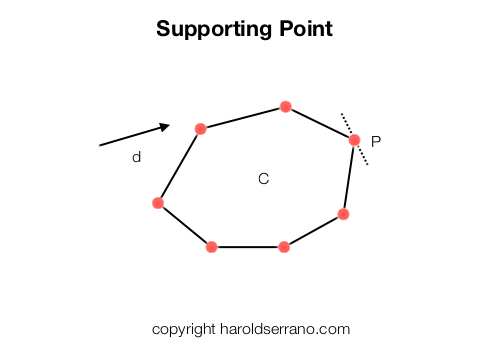
\includegraphics[width=.8\linewidth]{img/gjk/support.jpeg} } }
  \end{itemize}
\end{frame}

\begin{frame} {GJK: Gilbert-Johnson-Keerthi}
  \begin{itemize}
    \item<1> Somme de Minkowski :
      \only<1>{ \centerline { 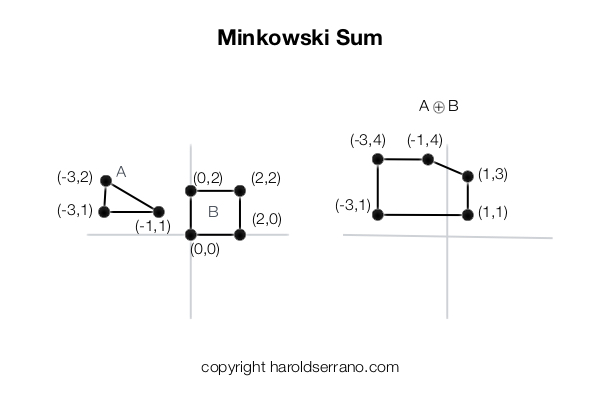
\includegraphics[width=.8\linewidth]{img/gjk/minkowski-sum.jpeg} } }
    \item<2> Diff\'erence de Minkowski :
      \only<2>{ \centerline { 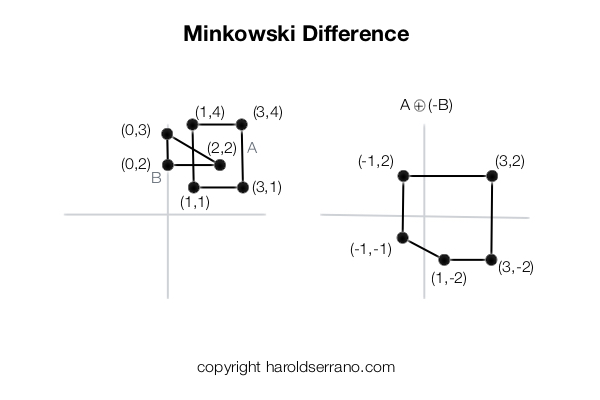
\includegraphics[width=.8\linewidth]{img/gjk/minkowski-diff.jpeg} } }
  \end{itemize}
\end{frame}

\begin{frame} {GJK: Gilbert-Johnson-Keerthi}
  \centerline{ 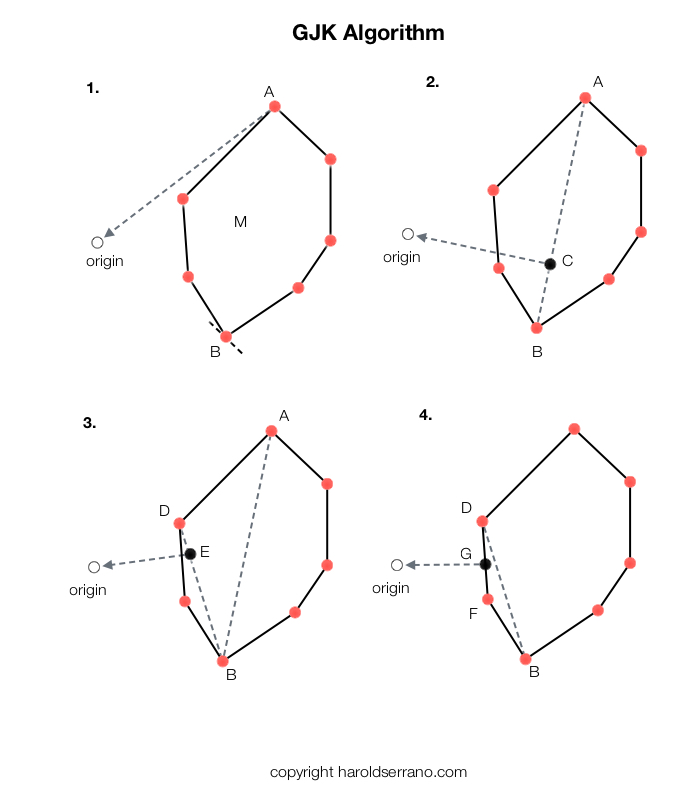
\includegraphics[width=.6\linewidth]{img/gjk/gjk.jpeg} }
\end{frame}
